\documentclass{article}

\usepackage[nonatbib]{neurips_2020}

\usepackage[utf8]{inputenc}
\usepackage[T1]{fontenc}
\usepackage{hyperref}
\usepackage{url}
\usepackage{booktabs}
\usepackage{amsfonts}
\usepackage{nicefrac}
\usepackage{microtype}
\usepackage{graphicx}
\graphicspath{{../plots/}{plots/}}

\title{Three Layers of LLM Inference: A Critical Reading of FlashAttention, Orca, and PagedAttention}

\author{%
  Anonymous Author \\
  Department of Computer Science \\
  \texttt{anonymous@example.edu} \\
}

\begin{document}

\maketitle

\begin{abstract}
Modern LLM inference systems have converged on a three-layer optimization stack: kernel design, batch scheduling, and memory management. This report critically examines one foundational paper from each layer --- FlashAttention~[1], Orca~[4], and PagedAttention~[5] --- and argues that the most influential subsequent work in inference systems has come not from extending any single layer, but from negotiating the tensions between them. Three such tensions are surfaced: FlashAttention's contiguous-KV assumption against PagedAttention's block indirection; Orca's iteration-level scheduling against PagedAttention's strict prefill/decode separation; and the implicit assumption across all three that prefill and decode share the same hardware. Each tension drove a wave of subsequent work, surveyed here. The critique is grounded in a reimplementation of the PagedAttention runtime, including a paged-decode Triton kernel modelled on vLLM's \texttt{paged\_attention\_v2} launcher, which forced confrontation with integration questions the original papers leave informal. Code: \url{https://github.com/VincentPit/MiniPageAttention}.
\end{abstract}

\section{Introduction}

LLM inference has emerged as a workload distinct from training, with its own economics and its own bottlenecks. The autoregressive structure of decoding produces three consistent friction points: the attention operator's per-token quadratic cost, the queue-management problem of serving heterogeneous requests on a fixed batch, and the KV cache's growing memory pressure. Three papers from 2022--2023 --- FlashAttention~[1], Orca~[4], and PagedAttention~[5] --- established what may now be called the canonical three-layer view of inference optimization: kernel, batching, and memory. They are standard reading and have produced standard implementations.

This report makes two claims. First, that each of the three papers is more interesting in its limits than in its main contribution: each rests on assumptions that hold in isolation but become load-bearing constraints when the three are stacked. Second, that the post-2023 explosion of inference systems work --- chunked prefill~[6], disaggregated serving~[7,8], radix-trie caching~[9], speculative decoding~[10] --- is best read as an attempt to reconcile incompatibilities the original three create at their interfaces.

To ground the discussion, I reimplemented a teaching version of the PagedAttention runtime from scratch --- a block-paged KV cache with refcounted prefix sharing, an Orca-style iteration-level scheduler driving it, and a custom paged-decode Triton kernel modelled on vLLM's \texttt{paged\_attention\_v2} CUDA launcher~[5].\footnote{Source: \url{https://github.com/VincentPit/MiniPageAttention}} The choice of all three papers, and not PagedAttention alone, is forced by this exercise rather than decorative: a block allocator is inert without a scheduler that consults its budget, and a paged cache is inert without a kernel that can dereference its block tables. Orca supplies the scheduler half and FlashAttention the kernel half, so a PagedAttention runtime that actually runs is necessarily a composition of all three --- which is exactly why the seams between them are where the report spends its time. Several of the critiques below were prompted by integration friction that is invisible at the paper level but loud at the implementation level.

\section{FlashAttention: IO-aware attention and its assumptions}

\paragraph{Contribution.} FlashAttention~[1] reframes attention as an IO-bound operator. Standard implementations materialize an $N \times N$ attention matrix in HBM; FlashAttention tiles $Q$, $K$, $V$ into SRAM-resident blocks and streams the softmax via online accumulators, producing the same output without holding the full attention matrix. The headline result is a 2--4$\times$ speedup and a memory cost that scales linearly rather than quadratically with sequence length. FlashAttention-2~[2] reordered the inner loop to put the iteration over $K/V$ on the outer axis, improving GPU occupancy. FlashAttention-3~[3] adapted the design to H100's asynchronous tensor cores and TMA.

\paragraph{Where the paper is stronger than its framing.} A subtler contribution than the IO framing is the demonstration that softmax can be computed in tiled fashion in a production-quality kernel without losing numerical precision. Online softmax was HPC folklore; FlashAttention productionized it and made it the default mental model for attention kernels.

\paragraph{Hardware specificity.} Block sizes derive from A100 SRAM (192~KB per SM). Naive porting to H100 (228~KB), MI300, and TPU v5 yields suboptimal tiles. FlashAttention-3 effectively re-derives the design for one new platform, and the result is significantly more complex. The IO-aware \emph{framing} is portable; the kernel is not.

\paragraph{The contiguous-KV assumption.} FlashAttention assumes the KV tensor is contiguous in HBM with one stride per axis. This holds in training and in basic inference but breaks under PagedAttention, where KV is fragmented across blocks. Composing FlashAttention with PagedAttention required follow-on work --- FlashInfer~[11], vLLM's custom \texttt{paged\_attention\_v2.cu} kernel, and FlashAttention-3's paged variant. None of these are anticipated by the original paper, but together they imply the kernel's shape is more brittle than the IO analysis suggests. The streaming-softmax trick survived; the data-layout assumptions did not.

\paragraph{Causal mask and backward-pass economics.} FlashAttention v1 handles causal masking by computing then masking to $-\infty$, which produces branch divergence in the inner loop. FA2 fixed this with a loop reorder, but the v1 paper presents masking as a footnote when in production it is the dominant case. Separately, the paper sells FlashAttention partly as a training optimization, but the backward pass requires recomputation, trading FLOPs for memory --- and for inference, which dominates production economics, this aspect is irrelevant. The training benchmarks in [1] are arguably the weakest part of the empirical case.

\paragraph{Net read.} FlashAttention is the right kernel for training and a starting point for inference. For inference at scale, it has been progressively replaced by descendants that preserve the streaming-softmax trick but discard the contiguous-KV assumption. The paper is foundational because of the trick, not the implementation.

\section{Orca: iteration-level scheduling, and what it does not say}

Orca is the batching layer of the stack and the paper my reimplementation leans on most directly outside PagedAttention itself: the continuous-batching scheduler behind the E5 result below is a teaching-scale version of its central mechanism, and building it is what made concrete the fact that a block allocator and an iteration-level scheduler are co-dependent --- the \emph{scheduling $\times$ memory budget} tension taken up later.

\paragraph{Contribution.} Orca~[4] attacks GPU utilization on an inference server. Static batching wastes compute when sequences finish at different times --- the longest sequence forces the rest to keep occupying batch slots. Orca's contribution is iteration-level scheduling: between forward passes, the scheduler drops finished sequences and admits new ones from a queue, holding the batch dimension constant on the model side. A complementary primitive, \emph{selective batching}, runs the prefill of newly-admitted sequences alongside in-progress decodes, which have radically different shapes ($T_\text{new}{=}N$ for prefill versus $T_\text{new}{=}1$ for decode).

\paragraph{Where it succeeds.} The reported throughput gains (3--7$\times$) have been reproduced repeatedly in vLLM, TGI, TensorRT-LLM, and SGLang. Continuous batching is now industry standard. The central insight --- that GPU-side batch composition can change \emph{without} losing the persistent KV state --- was non-obvious and is now load-bearing in every modern inference engine. My own continuous-batching reimplementation reproduced an end-to-end speedup of $\approx$1.33$\times$ (175 vs.\ 233 tok/s) on a 16-request mixed-length GPT-2 workload drawn from the \texttt{HuggingFaceH4/no\_robots} instruction-following dataset (prompt $p_{50}/p_{95}{=}27/173$ tokens, output $p_{50}/p_{95}{=}185/256$ tokens, capped at 256 to bound bench wall-time), greedy-identical to the static-batch baseline on all 16 requests, with no tuning at all --- a small fraction of Orca's reported gains, but the workload here is far smaller and far more uniform than Orca's, and the direction matches. Sweeping the workload (Figure~\ref{fig:e5}) shows the expected shape: the v2 advantage is roughly flat across batch size in this small-batch regime ($\approx$1.12--1.16$\times$ for $N{=}4$--$12$ at fixed variance) but widens sharply with prompt-length variance --- from $0.97\times$ at lognormal $\sigma{=}0.3$ (where v1 wastes almost nothing and scheduler overhead dominates) to $1.41\times$ at $\sigma{=}0.9$ --- variance being the condition under which v1's max-padded batch wastes the most compute.

\begin{figure}[t]
  \centering
  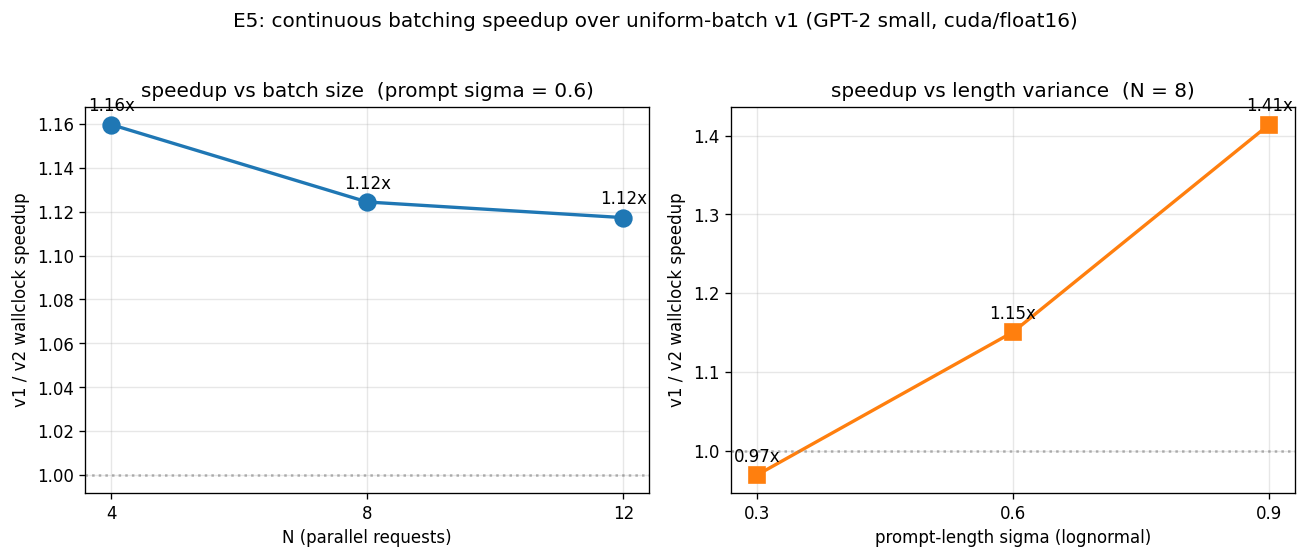
\includegraphics[width=\textwidth]{e5_speedup_sweep.png}
  \caption{Continuous-batching (v2) wall-clock speedup over a uniform static batch (v1), GPT-2 small (the run that produced the figure --- device and dtype --- is printed in the panel title). Left: speedup vs.\ number of parallel requests at fixed prompt-length variance. Right: speedup vs.\ prompt-length variance (lognormal $\sigma$) at fixed $N{=}8$. The single-point E5 result ($\approx$1.33$\times$ at $N{=}16$, mixed real prompt lengths) sits at the high end of this surface; the advantage shrinks --- and can invert ($0.97\times$ at $\sigma{=}0.3$) --- for small, uniform batches where v1 wastes little.}
  \label{fig:e5}
\end{figure}

\paragraph{Closed-source artifact.} Orca was implemented in a private Megatron-LM fork and never released. The paper motivates the design but does not contain enough detail to reproduce; vLLM's continuous batching, while inspired by Orca, makes several choices [5] does not discuss (admission ordering, block-aware throttling, EOS-based eviction). Reproducibility gaps in systems papers are easy to underweight when the canonical citation is ``Orca [4]'' rather than ``the vLLM continuous-batching scheduler.''

\paragraph{Selective batching's hidden cost.} Running a multi-token prefill alongside single-token decodes produces a step whose cost is dominated by the prefill. For long prefills (e.g., a 4k-token RAG context) and short decodes, the selective-batched step is essentially a prefill with hitchhikers --- decoders pay full attention cost for one token of progress. SARATHI~[6] formalized this as \emph{chunked prefill}: split prefills into chunks that interleave with multiple decode steps. Orca notes the issue but does not engage quantitatively; the chunked-prefill literature is the productive reading.

\paragraph{No memory model, no fairness model.} Orca assumes the KV cache is allocated contiguously and statically per slot. It says nothing about fragmentation, and its admission scheduler does not consult a KV budget --- only a slot count. PagedAttention picks up exactly this thread, but reading Orca alone leaves no sign that anything is missing. Independently, iteration-level scheduling is throughput-optimal but does not respect time-to-first-token (TTFT) under load. A request arriving when the batch is full waits an unbounded time for any sequence to finish. Orca acknowledges this in passing but offers no SLO model. Production systems retrofit priority queues and TTFT-aware admission, neither of which is discussed.

\paragraph{Net read.} Orca's core idea is correct and durable. Its specific proposed system is a starting point, not a destination. Reading Orca without reading SARATHI and the vLLM scheduler implementation tends to leave practitioners with an oversimplified mental model of how continuous batching is actually deployed.

\section{PagedAttention: virtual memory for the KV cache}

\paragraph{Contribution.} PagedAttention~[5] applies operating-system virtual-memory ideas to the KV cache. The cache is split into fixed-size blocks (typically 16 tokens $\times$ \texttt{n\_heads} $\times$ \texttt{head\_dim} per layer), and each sequence holds a \emph{block table} --- an indirection vector mapping logical positions to physical blocks. Three immediate consequences: external fragmentation is eliminated; parallel sampling and beam search can share prefix blocks via reference counting and copy-on-write; KV memory utilization approaches 100\% under realistic workloads where naive allocation wastes 60--80\%. The implementation in vLLM became one of the most-deployed inference engines in the field within a year of release. Replaying request traces through my BlockManager against a naive max-length allocator (Figure~\ref{fig:e2}) reproduces this gap directly: on a synthetic ShareGPT-shaped workload the naive-to-paged peak-occupancy ratio is 4.5$\times$, and on real conversation lengths streamed from \texttt{HuggingFaceH4/no\_robots} it is 5.6$\times$ --- the naive allocator's peak tracks the longest sequence ever admitted, while the paged peak tracks live token count.

\begin{figure}[t]
  \centering
  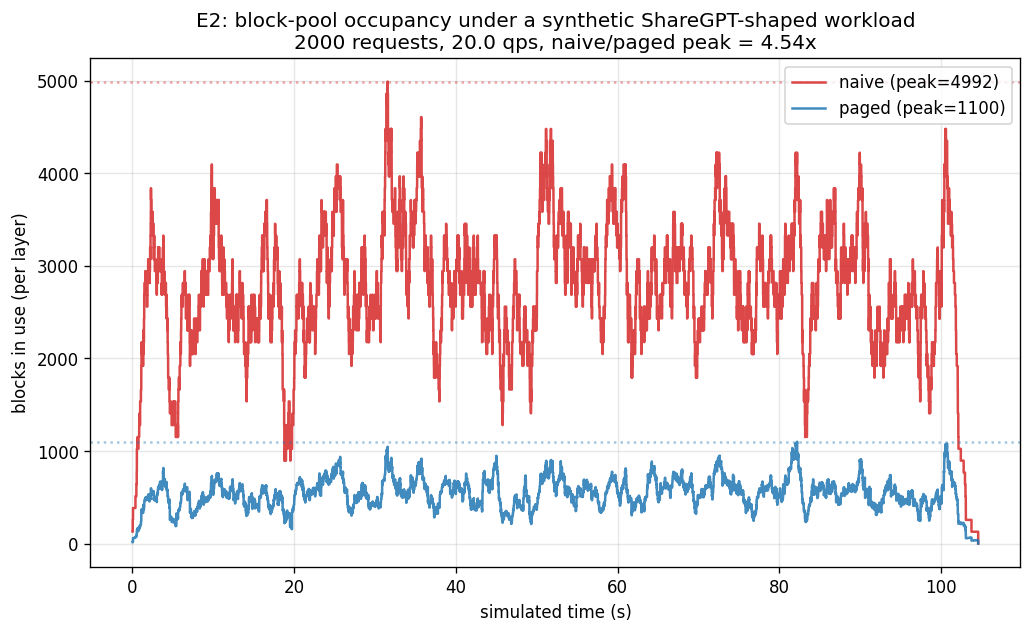
\includegraphics[width=0.49\textwidth]{e2_memory_timeseries.png}
  \hfill
  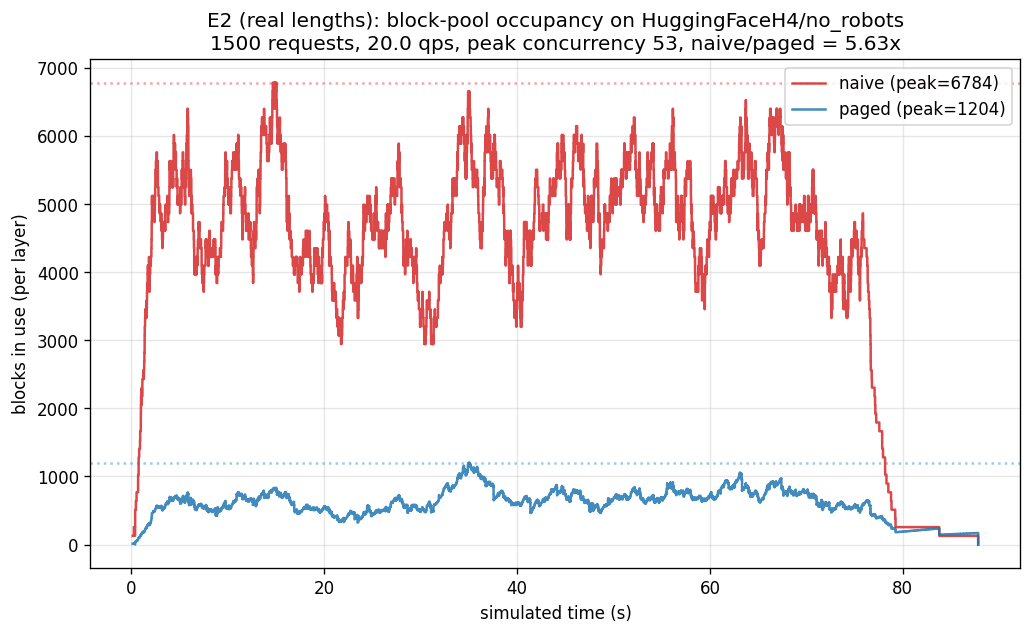
\includegraphics[width=0.49\textwidth]{e2_memory_real_lengths.png}
  \caption{Block-pool occupancy over time, paged (BlockManager) vs.\ naive per-slot max-length allocation, simulated at 20~qps. Left: a synthetic ShareGPT-shaped workload (2000 requests), naive/paged peak $= 4.5\times$. Right: real prompt+response lengths streamed from \texttt{HuggingFaceH4/no\_robots} (1500 requests, peak concurrency 53), ratio $= 5.6\times$. The naive curve is pinned near its worst case because every slot is sized for \texttt{max\_seq\_len}; the paged curve follows the live token count.}
  \label{fig:e2}
\end{figure}

\paragraph{Where the paper is right and important.} The fragmentation analysis is rigorous and the design decisions are well-motivated. The choice of block size $=16$ is empirically defensible --- large enough to amortize indirection cost, small enough to keep fragmentation under control. Refcounted COW for prefix sharing is exactly the right primitive; in my implementation, an 8-way parallel-sampling experiment from a 256-token prompt gave near-theoretical 8$\times$ prefill savings (and $\sim$5.7$\times$ end-to-end) with no special tuning, and the savings scale cleanly with the number of completions (Figure~\ref{fig:e3}): the post-prefill ratio sits right on the $y{=}N$ line, while after a few decode steps it bends below --- the shared prefix is amortized but the per-sequence decode blocks are not. The OS-virtual-memory metaphor is genuinely productive and not merely rhetorical.

\begin{figure}[t]
  \centering
  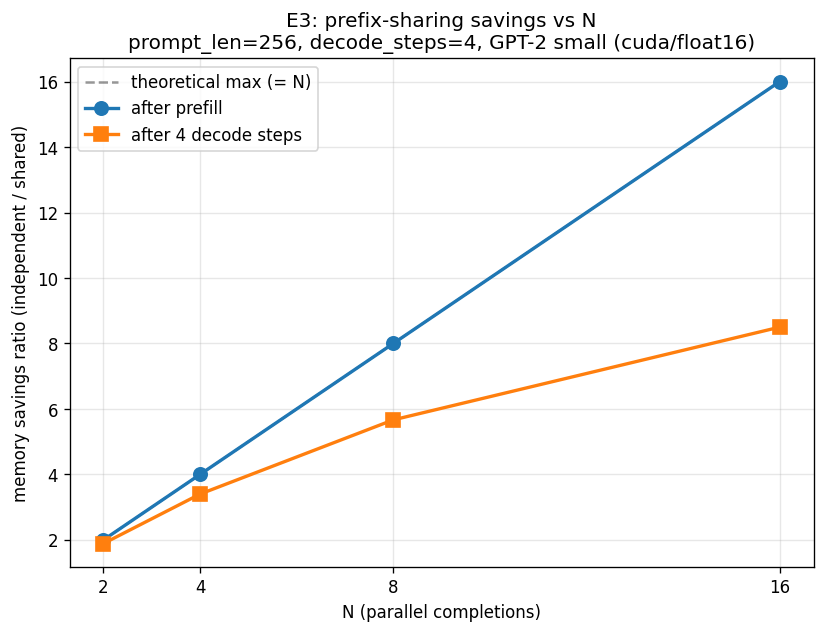
\includegraphics[width=0.62\textwidth]{e3_savings_vs_n.png}
  \caption{Prefix-sharing memory savings (independent / shared block-pool peak) vs.\ number of parallel completions $N$ from a single 256-token prompt, GPT-2 small. ``After prefill'' tracks the theoretical $y{=}N$ bound; ``after 4 decode steps'' falls below it because output blocks are allocated per sequence and are not shared.}
  \label{fig:e3}
\end{figure}

\paragraph{The kernel cost is paid every step.} Every K/V access goes through a block-table lookup. The custom CUDA kernel that ships with vLLM uses templated specialization across head sizes (32, 64, 80, 96, 112, 120, 128, 192, 256), block sizes (8, 16, 32), KV dtypes (fp16, fp8 e4m3, fp8 e5m2), and an \texttt{IS\_BLOCK\_SPARSE} flag --- a Cartesian product of compile-time configurations baked through nested macros. The paper mentions the kernel exists but does not discuss the engineering bill of compiling and shipping it. In my reimplementation, even the simpler decode-only Triton variant required autotuning over \texttt{num\_warps} $\times$ \texttt{num\_stages} to recover competitive throughput at small block sizes; the block-table indirection is decidedly not free, and a reader of [5] alone would not predict the eventual size of the kernel-engineering surface. The kernel reproduced \texttt{DynamicCache} token-for-token under greedy decoding on three of four probe prompts; on the fourth, a different floating-point reduction order flipped a near-tied logit after three tokens --- a reminder that ``exact'' attention is exact only up to accumulation order, which the paged layout silently changes.

\paragraph{Strict prefill/decode separation creates head-of-line blocking.} vLLM's scheduler runs prefills and decodes in separate forward passes. A long prefill --- common in RAG and tool-use workloads --- blocks all decode progress for hundreds of milliseconds. SARATHI~[6] and the broader chunked-prefill literature argue this is a more serious bottleneck than fragmentation for TTFT-sensitive workloads. PagedAttention's design implicitly endorses the separation; this was a defensible choice in 2023 and is now a known limitation.

\paragraph{Whole-block-only sharing.} Refcounting is at block granularity, so prefix sharing only helps when shared prefixes align with block boundaries. For a 16-token block and a 13-token shared prefix, sharing yields nothing. SGLang's RadixAttention~[9] generalizes to a radix tree with per-token granularity, at the cost of a more complex bookkeeping layer. The paper does not discuss this tradeoff and arguably underestimates how often real prefixes (system prompts, tool descriptions, formatting boilerplate) fall just under a block boundary.

\paragraph{Single-engine assumption.} The paper presents inference as monolithic --- one model, one engine, one GPU pool, prefill and decode on the same hardware. Splitwise~[8] and DistServe~[7] later showed that prefill and decode have radically different optimal hardware (compute-rich vs.\ memory-bandwidth-rich) and benefit from physical disaggregation. Block-table state then has to migrate across engines, which is awkward in PagedAttention's design.

\paragraph{Benchmarking caveats.} vLLM's headline gains are reported against a vLLM-authored Orca reproduction (the original being closed-source~[4]) and against FasterTransformer~[12]. The reported speedup is therefore between two community reimplementations, not between two production systems --- a subtlety easy to lose in citation chains.

\paragraph{Net read.} PagedAttention is the right answer to the fragmentation question it poses, and a partial answer to the broader scaling question, which binds to scheduler design, kernel composition, and disaggregation in ways the paper does not anticipate.

\section{The v2 launcher and what my implementation mirrors}

The launcher reproduced in Listing~\ref{lst:launcher} is the data-plane companion to PagedAttention. It runs no computation itself: every K/V access and every reduction lives inside the kernel the launcher dispatches to. Its substance is the dispatcher, and four nested layers of compile-time specialization fan out before a single CUDA kernel is launched.

\paragraph{Four-layer compile-time dispatch.} The outermost dispatcher \texttt{DISPATCH\_BY\_KV\_CACHE\_DTYPE} (in \texttt{cuda\_compat.h}) inspects \texttt{query.dtype()} and the \texttt{kv\_cache\_dtype} string to select the triple $(T, \texttt{CACHE\_T}, \texttt{KV\_DTYPE})$ --- $(\texttt{half}, \texttt{half}, \texttt{kAuto})$ for fp16 KV, $(\texttt{half}, \texttt{uint8\_t}, \texttt{kFp8E4M3})$ for fp8. The split between $T$ (compute dtype) and \texttt{CACHE\_T} (storage dtype) is what lets fp8 storage coexist with fp16 compute: the cache is dequantized inside the kernel using the per-tensor scales \texttt{k\_scale\_ptr} and \texttt{v\_scale\_ptr}. \texttt{CALL\_V2\_LAUNCHER\_BLOCK\_SIZE} then dispatches on \texttt{block\_size} $\in \{8, 16, 32\}$ --- the block size is a kernel constexpr because it sets the inner-loop trip count. \texttt{CALL\_V2\_LAUNCHER\_SPARSITY} branches on \texttt{IS\_BLOCK\_SPARSE} so the sparse path's extra index computations stay out of the dense fast path. Finally, the 9-way \texttt{switch} on \texttt{head\_size} inside \texttt{paged\_attention\_v2\_launcher} instantiates the kernel template on \texttt{HEAD\_SIZE}, which controls per-thread register pressure for the $Q$ vector and the $V$ accumulator. The Cartesian product is roughly $3 \times 3 \times 2 \times 9 \times 2 \approx 100$ specialized kernel instantiations per build, each compiled with no runtime branching on these axes --- the whole point of the dispatcher.

\paragraph{Inside the two kernels.} \texttt{LAUNCH\_PAGED\_ATTENTION\_V2} fires the two kernels that do the actual work. The partition kernel runs on a grid $(\text{num\_heads}, \text{num\_seqs}, \text{max\_num\_partitions})$ with \texttt{NUM\_THREADS}=128 (four warps) per block; each block handles one head of one sequence over one \texttt{PARTITION\_SIZE}=512-token slice. Threads cooperatively load $Q$ for $(b, h)$ into registers and walk the blocks of the assigned partition: \texttt{block\_tables\_ptr[b * max\_blocks + blk]} resolves to a physical block id, the kernel strides into \texttt{key\_cache\_ptr} via $\texttt{bid} \cdot \texttt{kv\_block\_stride} + h \cdot \texttt{kv\_head\_stride}$, and the warp computes $Q K^\top$ for the block's tokens. After the scale, optional ALiBi bias, and causal mask, the block tracks a partition-local online softmax (running max and exp-sum) and accumulates the weighted $V$. It writes three outputs into HBM scratch: \texttt{exp\_sums[b, h, p]} (partition denominator), \texttt{max\_logits[b, h, p]} (partition max), and \texttt{tmp\_out[b, h, p, :]} (un-normalized weighted $V$). The reduce kernel then runs on $(\text{num\_heads}, \text{num\_seqs})$, computes the global max $M = \max_p \texttt{max\_logits[b, h, p]}$, rescales each partition by $\alpha_p = \exp(\texttt{max\_logits[b, h, p]} - M)$, and forms $\texttt{out[b, h, :]} = (\sum_p \alpha_p \cdot \texttt{tmp\_out[b, h, p, :]}) / (\sum_p \alpha_p \cdot \texttt{exp\_sums[b, h, p]})$. This is exactly FlashAttention's online-softmax combine identity applied at partition granularity rather than tile granularity --- which is why v2 is best read as the paged adaptation of streaming attention, not a separate algorithm.

\paragraph{Pointer plumbing and the \texttt{x} factor.} The launcher's wide signature exists because the kernel does raw pointer arithmetic rather than multi-dimensional indexing. It reads \texttt{q\_stride = query.stride(0)}, \texttt{kv\_block\_stride = key\_cache.stride(0)}, and \texttt{kv\_head\_stride = key\_cache.stride(1)} from the tensors and passes them as integer arguments. The cache layout \texttt{[num\_blocks, num\_heads, head\_size/x, block\_size, x]} folds the head dimension into two strides --- \texttt{x} is the vector-load width (8 half-elements for the LDG.128 instruction). This layout is invisible to a reader of the PagedAttention paper but essential to coalesced memory access on the actual hardware. Triton tiles handle coalescing automatically, so my implementation drops the \texttt{/x} factor and uses the simpler \texttt{[blocks, block, heads, head]} layout that BlockManager already allocates.

Table~\ref{tab:correspondence} maps these primitives onto the Triton kernel in \texttt{gpu/paged\_attention\_kernel.py}. My implementation preserves the data plane --- block-table dereference, explicit strides, paged K/V layout, and FlashAttention's online-softmax accumulation (here run single-pass over the whole sequence per $(b, h)$ program, since GPT-2's contexts are short enough not to need the partition split; this is precisely the one piece of [1] that survives intact into a paged kernel) --- but discards the orthogonal complexity (fp8, ALiBi, block-sparse, tensor parallelism, the partition+reduce split) and replaces compile-time template specialization with Triton's runtime \texttt{constexpr} specialization at first call. The omitted axes are not conceptually difficult: fp8 needs dtype casts at load/store with per-tensor scales applied to the dot; ALiBi adds a position-dependent term inside the softmax; partition+reduce nearly doubles the kernel count. Collectively, they explain why vLLM ships roughly a hundred specialized C++ kernels while this implementation ships one Triton kernel for the $(D, \texttt{BLOCK\_SIZE}) = (64, 16)$ slice GPT-2 actually uses.

\begin{figure}[t]
\begin{verbatim}
void paged_attention_v2(...) {
  DISPATCH_BY_KV_CACHE_DTYPE(query.dtype(), kv_cache_dtype,    // (i)   dtype
                             CALL_V2_LAUNCHER_BLOCK_SIZE)
}

#define CALL_V2_LAUNCHER_BLOCK_SIZE(T, CACHE_T, KV_DTYPE)      \
  switch (block_size) {                                         \
    case  8: CALL_V2_LAUNCHER_SPARSITY(T, CACHE_T,  8, ...);    \
    case 16: CALL_V2_LAUNCHER_SPARSITY(T, CACHE_T, 16, ...);    \
    case 32: CALL_V2_LAUNCHER_SPARSITY(T, CACHE_T, 32, ...);    \
  }                                                            // (ii)  block

#define CALL_V2_LAUNCHER_SPARSITY(T, CACHE_T, BLOCK_SIZE, ...) \
  if (is_block_sparse) CALL_V2_LAUNCHER(..., true);             \
  else                 CALL_V2_LAUNCHER(..., false);           // (iii) sparse

// inside paged_attention_v2_launcher<T, CACHE_T, BLOCK_SIZE, KV_DTYPE, ...>
switch (head_size) {                                            // (iv)  head
  case  32: LAUNCH_PAGED_ATTENTION_V2( 32); break;
  case  64: LAUNCH_PAGED_ATTENTION_V2( 64); break;
  /* ... 80, 96, 112, 120, 128, 192 ... */
  case 256: LAUNCH_PAGED_ATTENTION_V2(256); break;
}

// LAUNCH_PAGED_ATTENTION_V2 fires two kernels:
//   paged_attention_v2_kernel        <<<(H,B,P), block, smem, stream>>>(...)
//   paged_attention_v2_reduce_kernel <<<(H,B),   block, smem, stream>>>(...)
\end{verbatim}
\caption{Condensed dispatch skeleton of vLLM's \texttt{paged\_attention\_v2} launcher. Four nested layers of compile-time specialization (i--iv) fan out before either CUDA kernel is launched, producing roughly $100$ specialized instantiations per build. The launcher fires a partition kernel followed by a reduce kernel that combines per-partition softmax statistics.}
\label{lst:launcher}
\end{figure}

\begin{table}[t]
  \caption{Correspondence between vLLM's \texttt{paged\_attention\_v2} launcher and the Triton kernel in \texttt{gpu/paged\_attention\_kernel.py}. The data-plane primitives transfer; the orthogonal-complexity axes (quantization, sparsity, parallelism, two-pass split) are intentionally absent.}
  \label{tab:correspondence}
  \centering
  \small
  \begin{tabular}{ll}
    \toprule
    vLLM launcher / kernel & My Triton implementation \\
    \midrule
    \texttt{paged\_attention\_v2\_kernel} (partitioned)            & \texttt{\_paged\_attn\_decode\_kernel} (single-pass) \\
    \texttt{paged\_attention\_v2\_reduce\_kernel}                  & subsumed by single-pass design \\
    \texttt{HEAD\_SIZE} template (9 specializations)               & Triton \texttt{constexpr D} \\
    \texttt{BLOCK\_SIZE} template (8/16/32)                        & Triton \texttt{constexpr BLOCK\_SIZE} \\
    \texttt{T, CACHE\_T, KV\_DTYPE} templates                      & Triton dtype inference (fp16/fp32) \\
    \texttt{block\_tables\_ptr}, \texttt{seq\_lens\_ptr}           & identical signature \\
    \texttt{q\_stride}, \texttt{kv\_block\_stride}, \texttt{kv\_head\_stride} & explicit kernel arguments \\
    \texttt{alibi\_slopes\_ptr}                                    & --- (GPT-2 uses learned position embeddings) \\
    \texttt{k\_scale\_ptr}, \texttt{v\_scale\_ptr} (fp8 scales)    & --- (no fp8 quantization) \\
    \texttt{IS\_BLOCK\_SPARSE}, \texttt{blocksparse\_*}            & --- \\
    \texttt{tp\_rank} (tensor parallelism)                         & --- (single engine) \\
    Cache layout \texttt{[blocks, heads, head/x, block, x]}        & \texttt{[blocks, block, heads, head]} \\
    \texttt{NUM\_THREADS=128}, \texttt{PARTITION\_SIZE=512}        & \texttt{num\_warps}, \texttt{num\_stages} autotuned \\
    \bottomrule
  \end{tabular}
\end{table}

\section{Three tensions and the work they motivated}

The three papers above are usually read as complementary --- and they are, in the sense that production systems use all three. They are also in tension on three specific axes, and most influential subsequent work has lived in those tensions.

\paragraph{Kernel $\times$ memory layout.} FlashAttention assumes contiguous KV; PagedAttention demands paged KV. Composing them requires either rewriting the kernel (FlashInfer~[11], vLLM's \texttt{paged\_attention\_v2.cu}) or relaxing contiguity in some other way. The ``v2'' partition-and-reduce kernel design --- partition the sequence into chunks, run streaming softmax per chunk, then a separate reduce kernel combines chunks --- is a direct synthesis: it preserves FlashAttention's online softmax while accepting PagedAttention's block indirection. It is also why kernel signatures in production paged-attention systems are dauntingly long, with templated specialization across nine head sizes, three block sizes, three KV dtypes, and a sparsity flag, all visible in the launcher I worked from.

\paragraph{Scheduling $\times$ memory budget.} Orca's iteration-level scheduler treats the batch slot as the resource; PagedAttention's allocator treats the block as the resource. Combining them requires the scheduler to consult a per-step block budget, which Orca did not anticipate and PagedAttention's paper does not deeply discuss. vLLM's swapping-out preemption (eviction of sequences whose KV no longer fits, with state migrated to CPU memory and reloaded later) and chunked-prefill-aware admission~[6] live in exactly this gap. FlexGen~[13] addresses an extreme version of the same gap when KV exceeds GPU memory entirely.

\paragraph{Single-engine $\times$ heterogeneous workload.} All three papers assume one engine. Real workloads have prefill-heavy and decode-heavy phases with different optimal hardware and different SLO sensitivities. Splitwise~[8] and DistServe~[7] split the engine; speculative decoding~[10] further muddies the picture by introducing draft-model rollbacks that interact non-trivially with paged KV (drafted tokens written to cache and then retracted). These designs preserve the per-layer ideas of the canonical three but change the system-level decomposition that all three implicitly assumed.

\section{Conclusion}

A common student reading of FlashAttention, Orca, and PagedAttention treats them as three separate optimizations to be plugged in independently. This report has argued instead that their interactions are where most recent progress lives. The three papers tell us how to make a single kernel fast, how to make a single batch flexible, and how to make a single allocator efficient. The harder question --- how those three optimizations cohere on a multi-tenant, multi-engine, mixed-workload inference platform --- is not answered by any of them, and the answers we have so far come from work that explicitly violates one assumption from each. For students of inference systems, the lesson is to read the three foundational papers in conjunction with their successors, not in isolation. The papers are foundational; they are not complete.

\section*{References}

\small

[1] Dao, T., Fu, D.Y., Ermon, S., Rudra, A.\ \& R\'e, C.\ (2022) FlashAttention: Fast and memory-efficient exact attention with IO-awareness. \emph{NeurIPS}.

[2] Dao, T.\ (2023) FlashAttention-2: Faster attention with better parallelism and work partitioning. \emph{arXiv:2307.08691}.

[3] Shah, J., Bikshandi, G., Zhang, Y., Thakkar, V., Ramani, P.\ \& Dao, T.\ (2024) FlashAttention-3: Fast and accurate attention with asynchrony and low-precision. \emph{arXiv:2407.08608}.

[4] Yu, G.-I., Jeong, J.S., Kim, G.-W., Kim, S.\ \& Chun, B.-G.\ (2022) Orca: A distributed serving system for transformer-based generative models. \emph{OSDI}.

[5] Kwon, W., Li, Z., Zhuang, S., Sheng, Y., Zheng, L., Yu, C.H., Gonzalez, J., Zhang, H.\ \& Stoica, I.\ (2023) Efficient memory management for large language model serving with PagedAttention. \emph{SOSP}.

[6] Agrawal, A., Kedia, N., Panwar, A., Mohan, J., Kwatra, N., Gulavani, B.S., Tumanov, A.\ \& Ramjee, R.\ (2024) Taming throughput-latency tradeoff in LLM inference with Sarathi-Serve. \emph{OSDI}.

[7] Zhong, Y., Liu, S., Chen, J., Hu, J., Zhu, Y., Liu, X., Jin, X.\ \& Zhang, H.\ (2024) DistServe: Disaggregating prefill and decoding for goodput-optimized large language model serving. \emph{OSDI}.

[8] Patel, P., Choukse, E., Zhang, C., Shah, A., Goiri, \'I., Maleki, S.\ \& Bianchini, R.\ (2024) Splitwise: Efficient generative LLM inference using phase splitting. \emph{ISCA}.

[9] Zheng, L., Yin, L., Xie, Z., Sun, C., Huang, J., Yu, C.H., Cao, S., Kozyrakis, C., Stoica, I., Gonzalez, J.E., Barrett, C.\ \& Sheng, Y.\ (2024) SGLang: Efficient execution of structured language model programs. \emph{NeurIPS}.

[10] Leviathan, Y., Kalman, M.\ \& Matias, Y.\ (2023) Fast inference from transformers via speculative decoding. \emph{ICML}.

[11] Ye, Z., Chen, L., Lai, R., Zhao, Y., Zheng, S., Shao, J., Hou, B., Jin, H., Zuo, Y., Yin, L., Chen, T.\ \& Ceze, L.\ (2024) FlashInfer: Efficient and customizable attention engine for LLM inference serving. \emph{arXiv:2501.01005}.

[12] NVIDIA (2023) FasterTransformer.\ \url{https://github.com/NVIDIA/FasterTransformer}.

[13] Sheng, Y., Zheng, L., Yuan, B., Li, Z., Ryabinin, M., Chen, B., Liang, P., R\'e, C., Stoica, I.\ \& Zhang, C.\ (2023) FlexGen: High-throughput generative inference of large language models with a single GPU. \emph{ICML}.

\end{document}
